\documentclass[a4paper, 10pt, english]{revtex4-2} %Add reprint for two columns

\usepackage[utf8]{inputenc}
\usepackage[english]{babel}

\usepackage{physics,amssymb}  % mathematical symbols (physics imports amsmath)
\usepackage{graphicx}         % include graphics such as plots
\usepackage{xcolor}           % set colors
\usepackage{hyperref}         % automagic cross-referencing (this is GODLIKE)
\usepackage{tikz}             % draw figures manually
%\usepackage{listings}         % display code
\usepackage{subfigure}        % imports a lot of cool and useful figure commands
\usepackage{array}
\usepackage{microtype}
\usepackage[export]{adjustbox}

\tolerance=1
\emergencystretch=\maxdimen
\hyphenpenalty=10000
\hbadness=10000

% defines the color of hyperref objects
% Blending two colors:  blue!80!black  =  80% blue and 20% black
\hypersetup{ % this is just my personal choice, feel free to change things
    colorlinks,
    linkcolor={red!50!black},
    citecolor={blue!50!black},
    urlcolor={blue!80!black}}

\newcommand{\txt}[1]{\text{#1}}
\newcommand{\parder}[2]{\frac{\partial #1}{\partial #2}}
\newcommand{\dder}[2]{\frac{\partial^2 #1}{\partial #2^2}}

\begin{document}
\vspace*{1.5cm}
\title{\LARGE Computational physics II: Project 1}
\author{Jon Aleksander Prøitz}
\date{\today}
\noaffiliation
\maketitle

Code used in the project can be found here:
\url{https://github.com/Jonaproitz/FYS4411-Project_1/}.
The code is logged in different branches coenciding with the problems in the project.

\section{\large Introduction}
    Theoritical studies of Bose-Einstein condensates in gases consisting of alkili atoms confined in magnetic or optical traps are often based off of the Gross-Pitaevskii equation. 
    Note that validity of these studies are dependent on the condition that the system is dilute, or in other words that the average distance between atoms is much larger than the range of the inter-atomic interactions. 
    Thus interactions of the system is largely dominated by two-body collisons wich are well described by the s-wave scattering length $a$.
    When defining the diluteness of a gas an important aspect is the gas parameter $x(r) = n(r)a^3$, where $n(r)$ is the local density of the system, and for low values of the average gas parameter $x_{av} = 10^{-3}$ the mean field Gross-Pitaevskii equation works excidingly well.
    Yet it has been shown experimentally that the local gas parameter can exceed this value by tuning the scattering length in the pressence of a Feshbach resonance.
    Thus improved many-body methods like Monte-Carlo calculations may be required.


    The goal of this project is to evaluate the ground state energy of a trapped, hard sphere Bose gas for different number of particles, using a specific trial wavefunction $\Psi_T$.
    We have used the Variational Monte Carlo method, starting with non-interacting particles in a spherical trap to check numerical data against analytical results.
    The trial wavefunction is used to study the sensitivity of condensate and non-condensate properties to the hard sphere radius and the number of particles.

    Our numerical studies start out with a simple Variational Monte Carlo method using the Metroplis algorithm to test the validity of our numerical data.
    We will then go on to add importance sampling based on the Fokker-Planck and Langevin equations, before adding a stochastic gradient descent algorithm to find optimal values of the trial wavefunction parameter $\alpha$.
    The result are then analyzed with the blocking technique.
    Finally we can then paralleize our program and start tackling the repulsive two-body problem.

    
\section{\large Quantum Monte Carlo theory}
    \subsection*{Quantum Monte Carlo}
        We approach our system with a numerical Monte Carlo calculation, using the Metroplis algorithm.
        In general for systems consisting of several particles, the integrals involved in the calculations of various expectation values are of a multi-dimensional characteristic and traditional methods such as Gauss-Legendre quadrature will not be suitable of our manybody system.
        The Monte Carlo calculation tests a variety of different states averaging the expectation value of the system, relying on the variational principle to yield the lowest states with a given symmetry.
        However in most cases, a wave function yields small values in large parts of configuration space, and a straightforward procedure which uses homogenously distributed random points in configuration space will most likely lead to poor results. 
        Therefore we will aplly the Metropolis algorithm combined with an importance sampling to more efficiently obtain the ground state energies.
        This is done with the goal that the regions in configuration space where the wavefunction has higher values will be sampled more efficiently.

        With this in mind the basic procedure of a Variational Monte Carlo calculations consists of:
        \begin{itemize}
            \item Constructing a trial wavefunction, for a manybody system consisting of $n$ particles lacated in postions $\mathbf{r = (\mathbf{r}_1,...,\mathbf{r}_2)}$. 
            The trial wavefunction depends on $m$ variational parameters $\mathbf{\alpha} = (\alpha_1,...,\alpha_m)$.
            \item Evaluating the expectation value of the Hamiltonian $H$.
            \item Vary $\mathbf{\alpha}$ according to some minimazation algorithm and return to the first step if we are not satisfied with the results.
        \end{itemize}
        

        In order to bring in the Monte Carlo machinery, we must define a probability density distribution (PDF). Using our ansatz for the trial wave function $\Psi_T(\mathbf{r}; \mathbf{\alpha})$ we define a trial PDF
        \begin{equation}
                P(\mathbf{r})
            =   \frac{\abs*{\Psi_T(\mathbf{r}; \mathbf{\alpha})}^2}{\int \abs*{\Psi_T(\mathbf{r}; \mathbf{\alpha})}^2 d\mathbf{r}}
        \end{equation}
        wich is our model for the probability distribution function. 
        The approximation to the expectation value of the Hamiltonian is now
        \begin{equation}
                \bar{E}[\mathbf{\alpha}]
            =   \frac{\int d\mathbf{r}\Psi_T^*(\mathbf{r};\mathbf{\alpha})H(\mathbf{r})\Psi_T(\mathbf{r};\mathbf{\alpha})}{\int d\mathbf{r} \Psi_T^*(\mathbf{r};\mathbf{\alpha})\Psi_T(\mathbf{r};\mathbf{\alpha})}
        \end{equation}


        We can then define a new quantity called the local energy
        \begin{equation}
                E_L(\mathbf{r};\mathbf{\alpha})
            =   \frac{1}{\Psi_T(\mathbf{r};\mathbf{\alpha})}H\Psi_T(\mathbf{r};\mathbf{\alpha})
        \end{equation}
        which, together with our trial PDF gives
        \begin{equation}
                \bar{E}[\mathbf{\alpha}]
            =   \int d\mathbf{r} P(\mathbf{r}) E_L(\mathbf{r};\mathbf{\alpha})
            \approx
                \frac{1}{N}\sum_{i=1}^N E_L(\mathbf{r};\mathbf{\alpha})
        \end{equation}
        where $N$ is the number of samples in the Monte Carlo calculation.
        The expression on the right hand side stems from Bernoulli's law of large numbers, which states that in the limit $N \to \infty$, the sample mean approaches the true mean.

        With the above in hand we can now define the main lines of our Monte Carlo algorithm, wich goes as:
        \begin{itemize}
            \item Fix the number of Monte Carlo steps with an initial set of positions $\mathbf{r}$ and variational parameters $\alpha$, then calculate $\abs{\Psi_T^\alpha(\mathbf{r})}^2$
            \item Initialise the energy and the variance and start the Monte Carlo calculation.
            \begin{itemize}
                \item Calculate a trial position $\mathbf{r}_p = \mathbf{r} + a \cdot step$ where $a$ is a random variable.
                \item Use the Metroplis algorithm to accept or reject this move, with a probalility of acceptance $w = P(\mathbf{r}_p) / P(\mathbf{r})$
                \item If the step is accepted, then we set $\mathbf{r} = \mathbf{r}_p$
                \item Update averages
            \end{itemize}
            \item Finish and compute final averages
        \end{itemize}
        Note that the jumping in space is governed by the variable step. 
        This is often referred to as the brute-force sampling and is normally replaced by what is called importance sampling.

    \subsection*{Importance sampling}
        For a diffusion process characterized by a time-dependent probability density $P(x, t)$ in one dimension the Fokker-Planck equation is
        \begin{equation}
                \parder{P}{t}
            =   D\parder{}{x}\left(\parder{}{x} - F\right)P(x, t)
        \end{equation}
        where $F$ is a drift term and $D$ is the diffusion coefficient.
        The new position in coordinate space is given as the solutions of the Langevin equation using Euler's method, namely, we go from the Langevin equation
        \begin{equation}
                \parder{x(t)}{t}
            =   DF(x(t)) + \eta
        \end{equation}
        with $\eta$ is a random variable, giving a new position
        \begin{equation}
                y
            =   x + DF(x)\Delta t + \xi \sqrt{\Delta t}
        \end{equation}
        where $\xi$ is gaussian random variable, $\Delta t$ is the chosen time step and the quantity $D$ is equal to $1/2$ in atomic units.
        Note that $\Delta t$ is viewed as a parameter. 
        In general values of $\Delta t \in [0.001, 0.01]$ yield rather stable values of the ground state energy.

        The process of isotropic diffusion characterized by a time-dependent probability density $P(x, t)$ approximately follows the Fokker-Planck equation given by
        \begin{equation}
            \parder{P}{t}
            =   \sum_i D\parder{}{\mathbf{x}_i}\left(\parder{}{\mathbf{x}_i} - \mathbf{F}_i\right)P(x, t)
        \end{equation}
        where $\mathbf{F}_i$ is the $i$th component of the drift term caused by an external potential, and $D$ is the diffusion coefficient. 
        The convergence to a stationary probability density can be obtained by setting the left hand side to zero such that the resulting equation will be satisfied if and only if all the terms of the sum are equal zero
        \begin{equation}
                \dder{P}{\mathbf{x}_i}
            =   P\parder{}{\mathbf{x}_i}\mathbf{F}_i + \mathbf{F}_i\parder{}{\mathbf{x}_i}P
        \end{equation}
        The drift vector should be of the form $\mathbf{F} = g(\mathbf{x})\parder{P}{\mathbf{x}}$. wich then gives
        \begin{equation}
            \dder{P}{\mathbf{x}_i}
            =   P\parder{g}{P}\left(\parder{P}{\mathbf{x}_i}\right)^2 + Pg\dder{P}{\mathbf{x}_i} + g\left(\parder{P}{\mathbf{x}_i}\right)^2
        \end{equation}
        The condition of stationary density means that the left hand side equals zero. 
        Thus the terms containing first and second derivatives have to cancel each other. 
        This is possible only when $g = 1/P$, wich yields
        \begin{equation}
                \mathbf{F}
            =   2\frac{1}{\Psi_T}\nabla\Psi_T
        \end{equation}
        which is known as the quantum force. 
        This term is responsible for "pushing" the random walker towards regions of the configuration space where the trial wave function has larger values. 
        This increases the efficiency of the simulation in contrast to the brute force Metropolis algorithm where the walker has the same probability of moving in every direction.

        The Fokker-Planck equation yields a transition probability given by the Green's function
        \begin{equation}
                G(y, x, \Delta t)
            =   \frac{1}{(4\pi D\Delta t)^{3N/2}} \exp(-(y - x - D\Delta t F(x))^2 / 4D\Delta t)
        \end{equation}
        which in turn means that our brute force Metropolis algorithm
        \begin{equation}
                A(y, x)
            =   \min(1, q(y, x))
        \end{equation}
        with $q(y, x) = \abs{\Psi_T(y)}^2/\abs{\Psi_T(x)}^2$ is now replaced by the Metropolis-Hastings algorithm
        \begin{equation}
                q(y, x)
            =   \frac{G(x, y, \Delta t)\abs{\Psi_T(y)}^2}{G(x, y, \Delta t)\abs{\Psi_T(x)}^2}
        \end{equation}

        
    \subsection*{Gradient descent}
        In general when doing Monte Carlo calculations, we end up computing the expectation value of the energy in terms of some parameters $\alpha_0, \alpha_1,..., \alpha_n$ and search for a minimum in this multi-variable parameter space.
        This leads to an energy minimization problem where we need the derivative of the energy as a function of the variational parameters.
        To find the derivatives of the local energy expectation value as function of the variational parameters, we can use the chain rule and the hermiticity of the Hamiltonian.
        Limiting ourself to one variable we then define
        \begin{equation}
                \bar{E}_\alpha
            =   \derivative{E_L[\alpha]}{\alpha}
        \end{equation}
        as the derivative of the energy with respect to the variational parameter $\alpha$. 
        We then  also define the derivative of the trial function with respect to the paramter $\alpha$
        \begin{equation}
                \bar{\Psi}_\alpha
            =   \derivative{\Psi[\alpha]}{\alpha}
        \end{equation}
        The elements of the gradient of the local energy are then
        \begin{equation}
                \bar{E}_\alpha
            =   2\left(\langle\frac{\bar{\Psi}_\alpha}{\Psi[\alpha]}E_L[\alpha]\rangle - \langle\frac{\bar{\Psi_\alpha}}{\Psi[\alpha]}\rangle\langle E_L[\alpha]\rangle\right)
        \end{equation}

        From a computational point of view this means that we need to compute the expectation values of
        \begin{equation}
            \langle \frac{\Psi_\alpha}{\Psi[\alpha]} E_L \rangle
        \end{equation}
        and
        \begin{equation}
            \langle\frac{\bar{\Psi_\alpha}}{\Psi[\alpha]}\rangle\langle E_L[\alpha]\rangle
        \end{equation}

        The basic idea of the gradient descent method is that a function $F(\mathbf{x}), \mathbf{x} \equiv (x_1, x_2, ..., x_n)$, decreases fastest if one goes from $\mathbf{x}$ in the direction of the negative gradient $-\nabla F(\mathbf{x})$.
        It can be shown that if
        \begin{equation}
                \mathbf{x}_{k+1}
            =   \mathbf{x}_k - \gamma_k\nabla F(\mathbf{x}_k)
        \end{equation}
        with $\gamma_k > 0$.
        If $\gamma_k$ is sufficiently small, then $F(\mathbf{x}_{k+1}) \leq F(\mathbf{x}_k)$. 
        This means that for a sufficiently small $\gamma_k$ we are always moving towards smaller function values, i.e a minimum.

        The previous observation is the basis of the steepest descent method, which is also referred to as just the Gradient Descent method. 
        Here we start with an initial guess $x_0$ for a minimum of $F$ and compute new approximations according to
        \begin{equation}
                \mathbf{x}_{k+1}
            =   \mathbf{x}_k - \gamma_k\nabla F(\mathbf{x}_k), \txt{ } k \geq 0
        \end{equation}
        The parameter $\gamma_k$ is also often referred to as the step length or the learning rate within the context of Machine Learning.

        Ideally the sequence $\{\mathbf{x}_k\}_{k=0}$ converges to a global minimum of the function $F$. 
        However in general we do not know if we are in a global or local minimum of the function. 
        In the special case when $F$ is a convex function, all local minima are also global minima, so in this case gradient descent can converge to the global solution. 
        The advantage of this scheme is that it is conceptually simple and straightforward to implement.
        However the method in this form has some severe limitations.

        In machine learing we are often faced with non-convex high dimensional cost functions with many local minima. 
        Since the Gradient Descent method is deterministic we will get stuck in a local minimum, if the method converges, unless we have a very good intial guess. 
        This also implies that the scheme is sensitive to the chosen initial condition.
        Note that the gradient is a function of $\mathbf{x} = (x_1, ..., x_n)$ which makes it expensive to compute numerically.
        The gradient descent method is also sensitive to the choice of learning rate $\gamma_k$. 
        This stems the fact that we are only guaranteed that $F(\mathbf{x}_{k+1}) \leq F(\mathbf{x}_k)$ for sufficiently small values of $\gamma_k$.
        The problem is to determine an optimal learning rate. 
        If the learning rate is chosen too small the method will take a long time to converge and if it is too large we can experience erratic behavior.
        Many of these shortcomings can be alleviated by introducing randomness. 
        One such method is that of Stochastic Gradient Descent.

    \subsection*{Resampling methods}
        Resampling methods involve repeatedly drawing samples from a training set and refitting a model of interest on each sample such that we obtain additional information about the fitted model.
        For example, in order to estimate the variability of a linear regression fit, we can repeatedly draw different samples from the training data, fit a linear regression to each new sample, and then examine the extent to which the resulting fits differ.
        Such an approach may allow us to obtain information that would not be available from fitting the model only once using the original training sample.

        Resampling methods are an important tool in modern statistics. 
        However these approaches can be computationally expensive, because they involve fitting the same statistical method multiple times using different subsets of the training data. 
        Yet, due to recent advances in computing power, the computational requirements of resampling methods generally are not prohibitive. 

        The reasons that that we choose to use these resampling methods are that we treat the computer simulations as experiments run numerically on a computer. This is espessially true for the Monte Carlo methods we have used in this project.
        We therefore analyse our results using the same statistics tools as we would use analysing experimental data.
        And as in all experiments, we are looking for expectation values and an estimate of how accurate they are, i.e. possible sources for errors.
        As in other experiments, these sources of errors come in two classes, statistical and systematical errors.
        Statistical errors can be estimated using standard tools from statistics, while systematical errors are method specific and must be treated differently from case to case.

        In this project we will use the Blocking method, made popular by Flyvbjerg and Pedersen (1989) and it has since become one of the main ways to estimate $V(\hat{\theta})$ for exactly one $\hat{\theta}$, namely $\hat{\theta} = \bar{X}$.
        The strength of the blocking method is when the number of observations, $n$ is large. 
        For instance for large $n$, the complexity of dependent bootstrapping scales poorly, but the blocking method does not, moreover, it becomes more accurate the larger $n$ is.

        In the Blocking method we assume $n = 2^d$ where $d$ is an integer greater than $1$ and $X_1, X_2, ..., X_n$ is a stationary asymptotically uncorrelated time series.
        Then by switching to vector notation by arranging $X_1, X_2, ..., X_n$ in an $n$-tuple, we can define
        \begin{equation}
                \hat{\mathbf{X}}
            =   (X_1, X_2, ..., X_n)
        \end{equation}

        We can now define blocking transformations. 
        The idea is to take the mean of subsequent pairs of elements from $\hat{\mathbf{X}}$ and form a new vector $\hat{\mathbf{X}}_1$.
        Continuing in the same way by taking the mean of subsequent pairs of elements of $\hat{\mathbf{X}}_1$ we obtain $\hat{\mathbf{X}}_2$, and so on.
        We then define $\hat{\mathbf{X}}_i$ by
        \begin{equation}
                (\hat{\mathbf{X}}_0)_k 
            \equiv
                (\hat{\mathbf{X}})_k
        \end{equation}
        and
        \begin{equation}
                (\hat{\mathbf{X}}_{i+1})_k
            \equiv
                \frac{1}{2}\left((\hat{\mathbf{X}}_i)_{2k-1} + (\hat{\mathbf{X}}_i)_{2k}\right)
            \txt{  for all  }
                1 \leq i \leq d - 1
        \end{equation}
        Where the quantity $\hat{\mathbf{X}}_k$ is subject to $k$ blocking transformations. 
        We now have $d$ vectors $\hat{\mathbf{X}}_0, \hat{\mathbf{X}}_1, ..., \hat{\mathbf{X}}_{d-1}$ containing the subsequent averages of observations. 
        It can then be shown that if the components of $\hat{\mathbf{X}}$ is a stationary time series, then the components of $\hat{\mathbf{X}}_i$ is also a stationary time series for all $i$ where $0 \leq i \leq d - 1$.
        Thus we can compute the autocovariance, the variance, sample mean, and number of observations for each $i$.
        Letting $\gamma_i$, $\sigma_i$ and $\bar{\mathbf{X}}_i$ denote the autocovariance, variance and average of the elements of $\hat{\mathbf{X}}_i$ and let $n_i$ be the number of elements of $\hat{\mathbf{X}}$.
        It then follows by induction that $n_i = n/2^i$.

        Using the definition of the blocking transformation and the distributive property of the covariance, it is clear that since $h = \abs{i - j}$ we can define
        \begin{equation*}
                \gamma_{k+1}(h)
            =   cov((X_{k+1})_i, (X_{k+1})_i)
        \end{equation*}
        \begin{equation*}
            =   \frac{1}{4} cov((X_k)_{2i-1} + (X_k)_{2i}, (X_k)_{2j-1} + (X_k)_{2j})
        \end{equation*}
        \begin{equation*}
            =   \frac{1}{2}\gamma_k (2h) + \frac{1}{2}\gamma_k(2h+1)h = 0
        \end{equation*}
        \begin{equation*}
            =   \frac{1}{4}\gamma_k(2h - 1) + \frac{1}{2}\gamma_k(2h) + \frac{1}{4}\gamma_k(2h + 1)
            \txt{ else}
        \end{equation*}
        The quantity $\hat{\mathbf{X}}$ is asymptotically uncorrelated by assumption, and $\hat{\mathbf{X}}_k$ is also asymptotically uncorrelated. 
        
        Let's turn our attention to the variance of the sample mean $V(\bar{X})$.
        We have
        \begin{equation}
                V(\bar{X}_k)
            =   \frac{\sigma_k^2}{n_k} + \frac{2}{n_k} \sum_{h=1}^{n_k - 1} \left(1 - \frac{h}{n_k}\right)\gamma_k(h)
            =   \frac{\sigma_k^2}{n_k} + e_k 
            \txt{ if }
                \gamma_k(0)
            =   \sigma_k^2
        \end{equation}
        Where $e_k$ is the truncation error:
        \begin{equation}
                e_k 
            =   \frac{2}{n_k} \sum_{h=1}^{n_k - 1} \left(1 - \frac{h}{n_k}\right)\gamma_k(h)
        \end{equation}
        We can now show that $V(\bar{X}_i) = V(\bar{X}j)$ for all $0 \leq i \leq d - 1$ and $0 \leq j \leq d - 1$.
        Thus
        \begin{equation}
                n_{j+1}\bar{X}_{j+1}
            =   \sum_{i=1}^{n_j+1} (\hat{\mathbf{X}}_{j+1})_i
            =   \frac{1}{2} \sum_{i=1}^{nj/2} (\hat{\mathbf{X}}_j)_{2i - 1} + (\hat{\mathbf{X}}_j)_{2i}
            =   \frac{n_j}{2}\bar{X}_j
            =   n_{j + 1} \bar{X}_j
        \end{equation}
        By repeated use of this equation we get $V(\bar{X}_i) = V(\bar{X}_0) = V(\bar{X})$ for all $0 \leq i \leq d - 1$.
        This has the consequence that 
        \begin{equation}
                V(\bar{X})
            =   \frac{\sigma_k^2}{n_k} + e_k 
            \txt{ for all }
                0 \leq k \leq d - 1
        \end{equation}

        Flyvbjerg and Petersen demonstrated that the sequence $\{e_k\}_{k=0}^{d-1}$ is decreasing, and conjecture that the term $e_k$ can be made as small as we would like by making $k$ sufficiently large. Thus we can apply blocking transformations until $e_k$ is sufficiently small, and then estimate $V(\bar{X})$ by $\hat{\sigma}_k^2 / n_k$.
        

\section{\large Analytic expressions}
    We represent our system with either a spherical (S), or elliptical (E) trap, given by
    \begin{equation}
            V_{ext}(\mathbf{r}) 
        =   \Bigg\{
        \begin{array}{ll}
            \frac{1}{2}m\omega_{ho}^2r^2 & (S)\\
        \strut
            \frac{1}{2}m[\omega_{ho}^2(x^2+y^2) + \omega_z^2z^2] & (E)
        \label{eq: trap_eqn}
        \end{array}
    \end{equation}
    in the spherical case $\omega_{ho}$ defines the trap potential, while for the elliptical case $\omega_{ho}$ defines the trap frequency in the $xy$-plane and $\omega_z$ is the trap frequency in the $z$-direction.
    The mean square vibrational amplitude of a single boson at $T=0K$ is $\langle x^2\rangle = \sqrt{\hbar/2m\omega_{ho}}$ such that the charecteristic length is $a_{ho} = \sqrt{\hbar/m\omega_{ho}}$.
    The two-body Hamiltonian of the system is
    \begin{equation}
            H
        =   \sum_i^N \left(\frac{-\hbar^2}{2m} \nabla_i^2 + V_\txt{ext}\right) + \sum_{i<j}^N V_\txt{int}
        \label{eq: Hamiltonian}
    \end{equation}
    with $N$ being the number of particles and the inter-boson interaction is represented by a pairwise repuslive potential
    \begin{equation}
        V_{int}(|\mathbf{r}_i-\mathbf{r}_j|) =  \Bigg\{
        \begin{array}{ll}
            \infty & {|\mathbf{r}_i-\mathbf{r}_j|} \leq {a}\\
            0 & {|\mathbf{r}_i-\mathbf{r}_j|} > {a}
        \end{array}
    \end{equation}
    where $a$ is the hard-core diameter of the bosons.
    The trial wavefunction for the ground state with $N$ atoms is given by
    \begin{equation}
        \Psi_T(\mathbf{r})=\Psi_T(\mathbf{r}_1, \mathbf{r}_2, \dots \mathbf{r}_N,\alpha,\beta)
        =\left[
        \prod_i g(\alpha,\beta,\mathbf{r}_i)
        \right]
        \left[
        \prod_{j<k}f(a,|\mathbf{r}_j-\mathbf{r}_k|)
        \right],
        \label{eq: trialwf}
    \end{equation}
    with 
    \begin{equation}
            g(\alpha, \beta, \mathbf{r}_i)
        =   exp\left[-\alpha\left(x_i^2+y_i^2+\beta z_i^2\right)\right]
    \end{equation}
    and
    \begin{equation}
            f(a,|\mathbf{r}_i-\mathbf{r}_j|)=\Bigg\{
        \begin{array}{ll}
            0 & {|\mathbf{r}_i-\mathbf{r}_j|} \leq {a}\\
            (1-\frac{a}{|\mathbf{r}_i-\mathbf{r}_j|}) & {|\mathbf{r}_i-\mathbf{r}_j|} > {a}.
        \end{array}
    \end{equation}
    \subsection*{Local energy}
        For non-interacting bosons we set $a=0$ in a spherical potential, $\beta=1$, such that the trial wavefunction can be written
        \begin{equation}
                \Psi_T(\mathbf{r})
            =   e^{-\alpha r^2}
            =   e^{-\alpha (x^2 + y^2 + z^2)}
        \end{equation}
        
        The local energy in one dimension is then given by the double derivative in one dimension
        \begin{equation}
                E_L 
            =   \frac{1}{\Psi_T}H\Psi_T
            =   \frac{1}{\Psi_T}\dder{\Psi_T}{x} + V_{ext}
            =   -2\alpha\frac{1}{\Psi_T}\parder{\Psi_T}{x}\left(x\Psi_T\right) + V_{ext}
            =   2\alpha{\left(2\alpha x^2 - 1\right)} + V_{ext}
        \end{equation}
        Denoting the vector $\mathbf{r} \equiv \mathbf{x} = (x_1, x_2, x_3)$, with $\nabla^2 = \sum_{i=1}\dder{}{x_i}$, we obtain the double derivative of a single boson in $d$ dimensions
        \begin{equation}
                \frac{1}{\Psi_T(\mathbf{x})} \sum_{i=1}^d \dder{\Psi_T(\mathbf{x})}{x_i}
            =   2\alpha\left(2\alpha\sum_{i=1}^dx_i^2 - d\right)
            =   2\alpha\left(2\alpha r^2 - d\right)
        \end{equation}
        Hence the local energy of the total system in $d$ dimensions with $N$ particles is given by
        \begin{equation}
                E_L
            =   \sum_i^N\left(\frac{-\hbar^2}{2m}2\alpha\left(2\alpha r_i^2 - d\right) + \frac{1}{2}m\omega_{ho}^2r_i^2\right)
            =   \sum_i^N\frac{d}{2}\hbar\omega_{ho}
            =   \frac{Nd}{2}\hbar\omega_{ho}
            \label{eq: localEnergy}
        \end{equation}
        here we have used $\alpha = 1/2a_{ho}^2$ and $a_{ho} = \sqrt{\hbar/m\omega_{ho}}$ in the second calculation.
        We note that setting $\hbar=\omega_{ho}=m=1$ gives $\alpha=1/2$.

    \subsection*{Drift force}
        Again denoting $\mathbf{r} \equiv \mathbf{x} = (x_1, x_2, x_3)$, the quantum force
        \begin{equation}
                \mathbf{F}
            =   \frac{2\nabla \Psi_T(\mathbf{x})}{\Psi_T(\mathbf{x})}
            =   \frac{2}{\Psi_T}\sum_{i=1}^d \hat{\mathbf{x}}_i\dder{}{x_i}e^{-\alpha x^2}
            =   -4\alpha \sum_{i=1}^d x_i \hat{\mathbf{x}_i}
        \end{equation}

    \subsection*{Two-body interaction}
        Define $g(\alpha, \beta, \mathbf{r}_i) = \phi(\mathbf{r}_i)$ and $r_{jm} = |\mathbf{r}_j - \mathbf{r}_m|$, such that
        \begin{equation}
                \Psi_T 
            =   \left[\prod_i\phi(\mathbf{r}_i)\right] e^{\sum_{j<m} \ln{f(r_{jm})}}
            =   \left[\prod_i\phi(\mathbf{r}_i)\right] e^{\sum_{j<m} u(r_{jm})}
        \end{equation}
        with $u(r_{jm}) = \ln{f(r_{jm})}$. The derivative of particle $k$ is then
        \begin{equation}
                \nabla_k\Psi_T 
            =   \nabla_k\left[\prod_i \phi(\mathbf{r}_i)\right]e^{\sum_{j<m} u(_{jm})} + \left[\prod_i\phi(\mathbf{r}_i)\right] \nabla_k\left(e^{\sum_{j<m} u(r_{jm})}\right)
        \end{equation}
        we note that in the frist term only particle $k$ is affected by the derivation, such that
        \begin{equation}
                \nabla_k\prod_i \phi(\mathbf{r}_i) 
            =   \nabla_k\phi(\mathbf{r}_i)\left[\prod_{i\neq k}\phi(\mathbf{r}_i)\right]
            \label{eq: derphi}
        \end{equation}
        while the second term
        \begin{equation}
                    \nabla_k\left(e^{\sum_{j<m} u(r_{jm})}\right)
                =   e^{\sum_{j<m} u(r_{jm})} \nabla_k\sum_{j<m}u(r_{jm})
                =   e^{\sum_{j<m} u(r_{jm})} \sum_{l \neq k}\nabla_k u(r_{kl})
                \label{eq: dere}
        \end{equation}
        such that
        \begin{equation}
                \nabla_k\Psi_T 
            =   \nabla_k\phi(\mathbf{r}_k)\left[\prod_{i \neq k}\phi(\mathbf{r}_i)\right] e^{\sum_{j<m} u(r_{jm})} + \left[\prod_i\phi(\mathbf{r}_i)\right] e^{\sum_{j<m} u(r_{jm})} \sum_{l \neq k}\nabla_k u(r_{kl})
            \label{eq: first der}
        \end{equation}     

        To find the double derivative we start by derivating the first term of eq \ref*{eq: first der}
        \begin{equation}
                \nabla_k\left(\nabla_k\phi(\mathbf{r}_k)\left[\prod_{i\neq k}\phi(\mathbf{r}_i)\right] e^{\sum_{j<m} u(r_{jm})}\right)
            =   \left[\prod_{i\neq k}\phi(\mathbf{r}_i)\right] e^{\sum_{j<m} u(r_{jm})} \nabla_k^2\phi(\mathbf{r}_k) + \nabla_k\phi(\mathbf{r}_k)\left[\prod_{i\neq k}\phi(\mathbf{r}_i)\right] \nabla_k e^{\sum_{j<m} u(r_{jm})}
            \label{eq: more derivations}
        \end{equation}
        the first term of eq \ref*{eq: more derivations} is then
        \begin{equation}
                \frac{\left[\prod_{i\neq k}\phi(\mathbf{r}_i)\right] e^{\sum_{j<m} u(r_{jm})}}{\Psi_T} \nabla_k^2 \phi(\mathbf{r}_k)
            =   \frac{\left[\prod_{i\neq k}\phi(\mathbf{r}_i)\right] e^{\sum_{j<m} u(r_{jm})}}{\phi(\mathbf{r}_k)\left[\prod_{i\neq k}\phi(\mathbf{r}_i)\right] e^{\sum_{j<m} u(r_{jm})}} \nabla_k^2 \phi(\mathbf{r}_k)
            =   \frac{1}{\phi(\mathbf{r}_k)} \nabla_k^2 \phi(\mathbf{r}_k)
        \end{equation}
        Using eq \ref*{eq: dere} we find that the second term of eq \ref*{eq: more derivations}
        \begin{equation}
                \frac{\nabla_k \phi(\mathbf{r}_k) \left[\prod_{i\neq k}\phi(\mathbf{r}_i)\right]}{\Psi_T} \nabla_k e^{\sum_{j<m} u(r_{jm})}
            =   \frac{\nabla_k \phi(\mathbf{r}_k)}{\phi(\mathbf{r}_k)} \sum_{l \neq k}\nabla_k u(r_{kl})
        \end{equation}
        moving on to the second term of eq \ref*{eq: first der}
        \begin{align}
        \begin{split}
                &\nabla_k\left(\left[\prod_i\phi(\mathbf{r}_i)\right] e^{\sum_{j<m} u(r_{jm})} \sum_{l \neq k}\nabla_k u(r_{kl})\right)\\
            =   &e^{\sum_{j<m} u(r_{jm})} \sum_{l \neq k}\nabla_k u(r_{kl}) \nabla_k \left[\prod_i\phi(\mathbf{r}_i)\right] 
                + \left[\prod_i\phi(\mathbf{r}_i)\right] \sum_{l \neq k}\nabla_k u(r_{kl}) \nabla_k e^{\sum_{j<m} u(r_{jm})}\\
            &+  \left[\prod_i\phi(\mathbf{r}_i)\right] e^{\sum_{j<m} u(r_{jm})} \nabla_k \sum_{l \neq k}\nabla_k u(r_{kl})
            \label{eq: second der}
        \end{split}
        \end{align}
        we find the first term of eq \ref*{eq: second der}
        \begin{equation}
                \frac{1}{\Psi_T} e^{\sum_{j<m} u(r_{jm})} \sum_{l \neq k}\nabla_k u(r_{kl}) \nabla_k \left[\prod_i\phi(\mathbf{r}_i)\right]
            =   \frac{\nabla_k \phi(\mathbf{r}_k)}{\phi(\mathbf{r}_k)} \sum_{l \neq k}\nabla_k u(r_{kl})
        \end{equation}
        then the second term
        \begin{equation}
                \frac{1}{\Psi_T}\left[\prod_i\phi(\mathbf{r}_i)\right] \sum_{l \neq k}\nabla_k u(r_{kl}) \nabla_k e^{\sum_{j<m} u(r_{jm})}
            =   \left(\sum_{l \neq k}\nabla_k u(r_{kl})\right) \left(\sum_{i \neq k}\nabla_k u(r_{ki})\right)
        \end{equation}
        and lastly the third term
        \begin{equation}
                \frac{1}{\Psi_T}\left[\prod_i\phi(\mathbf{r}_i)\right] e^{\sum_{j<m} u(r_{jm})} \nabla_k \sum_{l \neq k}\nabla_k u(r_{kl})
            =   \sum_{l \neq k} \nabla_k^2 u(r_{kl})
        \end{equation}

        Now with the realtions
        \begin{equation}
                \nabla_k u(r_{ki})
            =   \frac{\mathbf{r}_k - \mathbf{r}_i}{r_{ki}}u'(r_{ki})
        \end{equation}
        and
        \begin{equation}
                \nabla_k^2 u(r_{ki})
            =   u''(r_{ki}) + \frac{2}{r_{ki}}u'(r_{ki})
        \end{equation}
        we can find the second derivative
        \begin{align}
        \begin{split}
                \frac{1}{\Psi_T} \nabla_k^2 \Psi_T
            =   &\frac{\nabla_k^2 \phi(\mathbf{r}_k)}{\phi(\mathbf{r}_k)} 
                + 2\frac{\nabla_k \phi(\mathbf{r}_k)}{\phi(\mathbf{r}_k)} \sum_{j \neq k} \frac{\mathbf{r}_k - \mathbf{r}_j}{r_{kl}}u'(r_{kj}) \\
                &+ \sum_{j \neq k}\sum_{i \neq k} \frac{(\mathbf{r}_k - \mathbf{r}_j)(\mathbf{r}_k - \mathbf{r}_i)}{r_{kj}r_{ki}}u'(r_{kj})u'(r_{ki})
                + \sum_{j \neq k} u''(r_{kj}) + \frac{2}{r_{kj}}u'(r_{kj})
        \end{split}
        \label{eq: doubleder}
        \end{align}

        Then using 
        \begin{equation}
                u'(r_{kj})
            =   \derivative{\ln(f(a, r_{kj}))}{r_{kj}}
            =   \frac{1}{f(a, r_{kj})} f'(a,r_{kj})
            =   \frac{a}{r_{kj}^2}\frac{1}{f(a, r{kj})}
        \end{equation}
        and
        \begin{equation}
                u''(r_{kj})
            =   - \left(2\frac{a}{r_{kj}^3}\frac{1}{f(a, r_{kj})} + \frac{a^2}{r_{kj}^4}\frac{1}{f^2(a, r_{kj})}\right)
        \end{equation}
        we can rewrite equaton \ref{eq: doubleder}
        \begin{align}
        \begin{split}
                \frac{1}{\Psi_T} \nabla_k^2 \Psi_T
            =   &\frac{\nabla_k^2 \phi(\mathbf{r}_k)}{\phi(\mathbf{r}_k)}
                - 4 \left(x_k\mathbf{\hat{x}} + y_k\mathbf{\hat{y}} + \beta z_k\mathbf{\hat{z}}\right) \sum_{k \neq j}(\mathbf{r}_k - \mathbf{r}_j)\frac{a}{r_{kj}^3}\frac{1}{f(a, r_{kj})} \\
                &+ \sum_{k\neq j}\sum_{k\neq i} (\mathbf{r}_k - \mathbf{r}_j)(\mathbf{r}_k - \mathbf{r}_i) \frac{a}{r_{kj}^3} \frac{a}{r_{ki}^3} \frac{1}{f(a, r_{kj})f(a, r_{ki})}
                - \sum_{k \neq j}\frac{a^2}{r_{kj}^4}\frac{1}{f^2(a, r_{kj})}
        \end{split}
        \end{align}

    Lastly going from $r \to r/a_{ho}$ we can rewrite the elliptical Hamiltonian
    \begin{align*}
            H 
        =   \sum_{i=1}^N \left(\frac{-\hbar^2}{2m}\nabla_i^2 + \frac{1}{2}m\left[\omega_{ho}^2(x^2 + y^2) + \omega_z^2 z^2\right]\right) + \sum_{i < j} V_{int}(\abs{\mathbf{r}_i - \mathbf{r}_j}) \\
        \to
            H
        =   \sum_{i=1}^{N} \left(\frac{-\hbar^2}{2m}\frac{\nabla_i^2}{a_{ho}^2} + \frac{a_{ho}^2}{2}m\left[\omega_{ho}^2(x^2 + y^2) + \omega_z^2 z^2\right]\right) + \sum_{i < j} V_{int}(\abs{\mathbf{r}_i - \mathbf{r}_j}) \\
        =   \sum_{i=1}^{N} \left(\frac{-\hbar \omega_{ho}}{2} \nabla_i^2 + \frac{\hbar \omega_{ho}}{2}\left[x^2 + y^2 + \omega_{ho} \gamma^2 z^2\right]\right) + \sum_{i < j} V_{int}(\abs{\mathbf{r}_i - \mathbf{r}_j})
    \end{align*}
    where we have used $a_{ho} = \sqrt{\hbar / m\omega_{ho}}$ and $\gamma = \omega_z/\omega_{ho}$.
    In units $\hbar\omega_{ho}$ the Hamiltonian can therefore be written
    \begin{align}
    \begin{split}
            H 
        =   \sum_{i=1}^{N} \left(\frac{-1}{2} \nabla_i^2 + \frac{1}{2}\left[x^2 + y^2 + \omega_{ho} \gamma^2 z^2\right]\right) + \sum_{i < j} V_{int}(\abs{\mathbf{r}_i - \mathbf{r}_j}) \\
        =   \frac{1}{2} \sum_{i=1}^{N} \left(-\nabla_i^2 + x^2 + y^2 + \omega_{ho} \gamma^2 z^2\right) + \sum_{i < j} V_{int}(\abs{\mathbf{r}_i - \mathbf{r}_j})
    \end{split}
    \end{align}


    \subsection*{Onebody densities}
        The onebody density for $N$ particles is given by
        \begin{equation}
                \rho(\mathbf{r}_1)
            =   N \int \prod_{i=2}^{N} d^3\mathbf{r}_i \abs{\Psi_T(\mathbf{r}_1, \mathbf{r}_2, ..., \mathbf{r}_N)}^2
        \end{equation}
        Inserting our trial wavefunction from the harmonic oscillator case
        \begin{equation}
                \rho(\mathbf{r}_1)
            =   N phi^2(\mathbf{r}_1) \int \prod_{i=2}^{N} d^3\mathbf{r}_i \phi^2(\mathbf{r}_i) \prod_{j < i} f^2(a, \abs{\mathbf{r}_i - \mathbf{r}_j})
        \end{equation}
        Limiting ourselves to two particles, we can see that in the non-interacting case the onebody density reduces to 
        \begin{equation}
                \rho(\mathbf{r}_1)
            =   2 \phi^2(\mathbf{r}_1) \int d^3\mathbf{r}_2 \phi^2(\mathbf{r}_2)
        \end{equation}
        while in the interacting case 
        \begin{equation}
                \rho(\mathbf{r}_1)
            =   2 \phi^2(\mathbf{r}_1) \int d^3\mathbf{r}_2 \phi^2(\mathbf{r}_2) f^2(a, \abs{\mathbf{r}_1 - \mathbf{r}_2})
        \end{equation}


\section{\large Numerical approach}
    The starting point of our numerical calculatons is the Monte Carlo calculation desrcibed in section II.
    To build the numerical structure of our program, we use the spherical trap described eq: \ref{eq: trap_eqn}.
    With non-interacting bosons as our particle of choice.
    The Metropolis algorithm is used on a single particle in a single dimension at a time and sampled once every particle in every dimension has undergone i single Monte Carlo step.
    When all Monte Carlo steps are completed we calculate the mean energy and variance of the system for a given parameter $\alpha$ and redo the calculation with different values of $\alpha$ to get an understanding of how the system changes with this parameter.
    
    The calculations are run for $n = 1$, $n = 10$, $n=100$ and $n = 500$, where $n$ denotes the number of particles, with the parameter $\alpha \in [0.2, 0.9]$.
    The results of these calcualtions are shown in figures \ref{fig: B1}, \ref{fig: B10}, \ref{fig: B100} and \ref{fig: B500}.
    For non-interacting bosons, using natural units, we expect the to find the minimum energies for $\alpha = 0.5$.
    This matches all three of our calculations, and we note that the variance for $alpha = 0.5$ is $0$ wich is also to be expected from eq \ref*{eq: localEnergy}.
    \def\imwidth{0.49\textwidth}
    \begin{figure}[!ht]
        \centering
        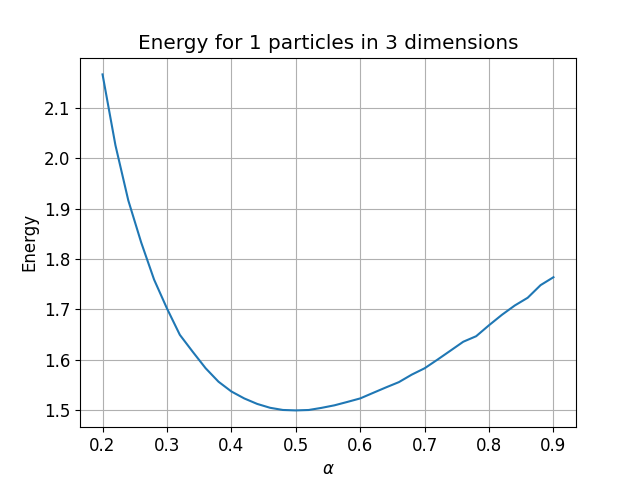
\includegraphics[width=\imwidth]{figures/Energy_B_1.png}
        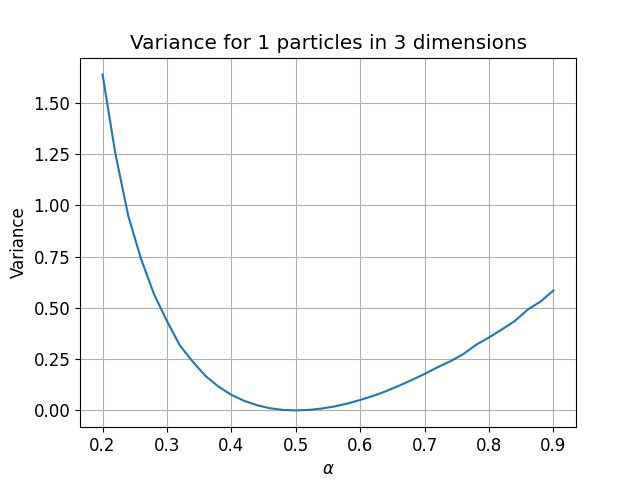
\includegraphics[width=\imwidth]{figures/Varience_B_1.png}
        \caption{Calcluated energy and variance using the Monte Carlo calculations for different values of the parameter $\alpha$ for $1$ non-interacing boson in a spherical trap.}
        \label{fig: B1}
    \end{figure}

    \begin{figure}[!ht]
        \centering
        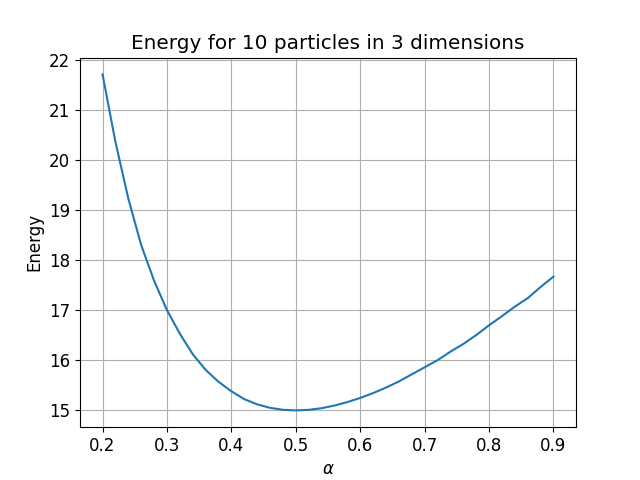
\includegraphics[width=\imwidth]{figures/Energy_B_10.png}
        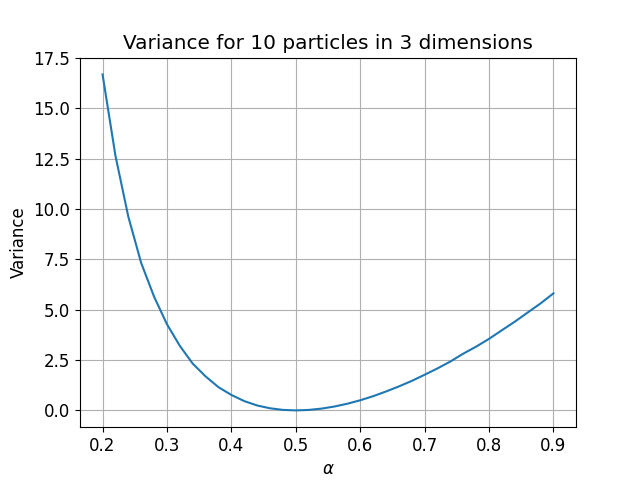
\includegraphics[width=\imwidth]{figures/Varience_B_10.png}
        \caption{Calcluated energy and variance using the Monte Carlo calculations for different values of the parameter $\alpha$ for $10$ non-interacing bosons in a spherical trap.}
        \label{fig: B10}
    \end{figure}

    \begin{figure}[!ht]
        \centering
        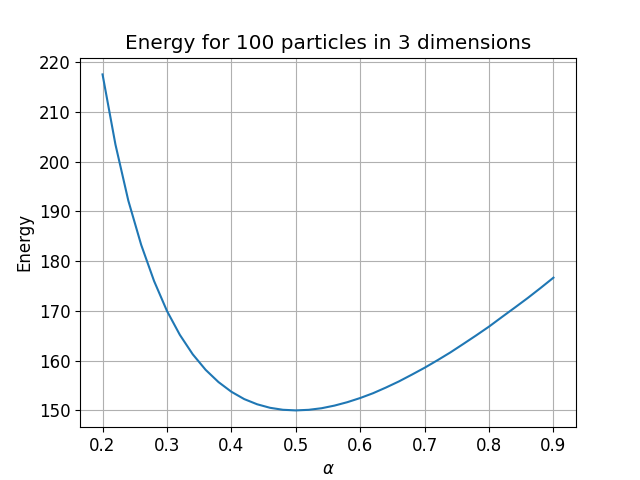
\includegraphics[width=\imwidth]{figures/Energy_B_100.png}
        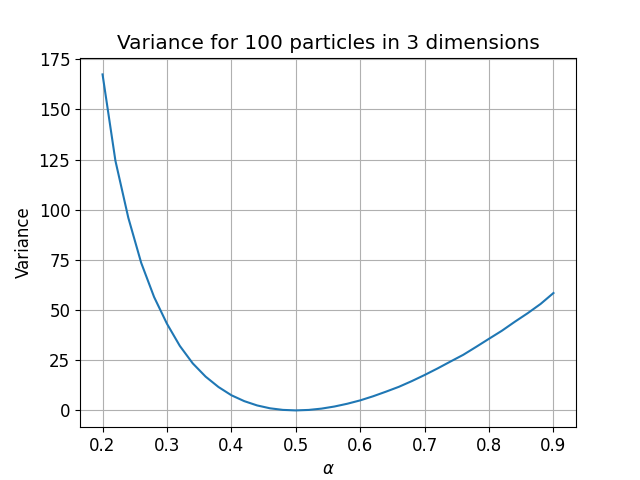
\includegraphics[width=\imwidth]{figures/Varience_B_100.png}
        \caption{Calcluated energy and variance using the Monte Carlo calculations for different values of the parameter $\alpha$ for $100$ non-interacing bosons in a spherical trap.}
        \label{fig: B100}
    \end{figure}
    
    \begin{figure}[!ht]
        \centering
        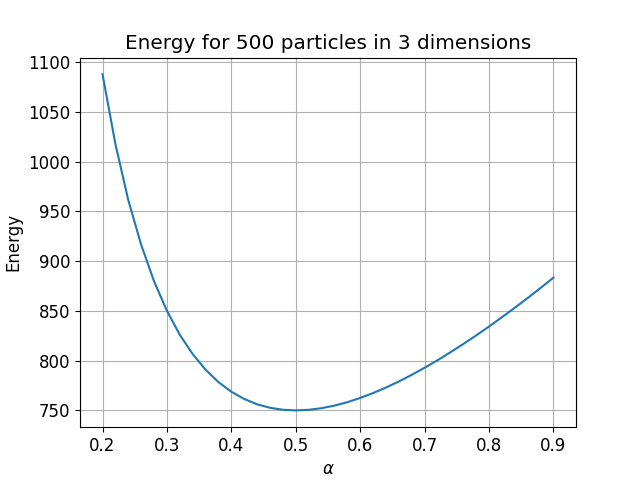
\includegraphics[width=\imwidth]{figures/Energy_B_500.png}
        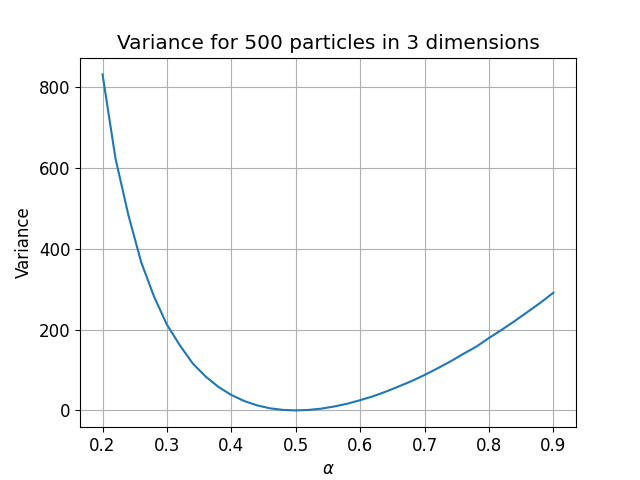
\includegraphics[width=\imwidth]{figures/Varience_B_500.png}
        \caption{Calcluated energy and variance using the Monte Carlo calculations for different values of the parameter $\alpha$ for $500$ non-interacing bosons in a spherical trap.}
        \label{fig: B500}
    \end{figure}\newpage\newpage
    

    The next goal is to implement importance sampling.
    This is done using a quantum force based on the Fokker-Planck and Langevin equations.
    In contrast to the brute force Monte Carlo calculation used previously, the importance sampling adds an "incentive" for the particles to move towards the areas where the trial wave function has greater values, as described in section II.
    The implementation of importance sampling to our calculations allows us to more efficiently sample the areas in coordinate space where the trial wavefunction is greater.
    Thus we aim to find the same ground state energies as with the brute force calculations but with fewer steps needed.

    The calculations are again run for $n = 1$, $n = 10$, $n=100$ and $n=500$ with the parameter $\alpha \in [0.2, 0.9]$.
    With the new results shown in figures \ref{fig: C1}, \ref{fig: C10}, \ref{fig: C100} and \ref{fig: C500}.
    Comparing these to figures \ref{fig: B1}, \ref{fig: B10}, \ref{fig: B100} and \ref{fig: B500} we note the great simularities and same overall results from the brute force Monte Carlo calculations.
    The mayor difference between the importance sampling and the brute force way is the number of Monte Carlo cycles used.
    In the brute force scenario we have used $10^6$ cycles while when using importance sampling we have used $10^5$ cycles.
    This naturally leads to lower times spent on these calculations, this is shown in table \ref{table: time spent}.
    \begin{figure}[!ht]
        \centering
        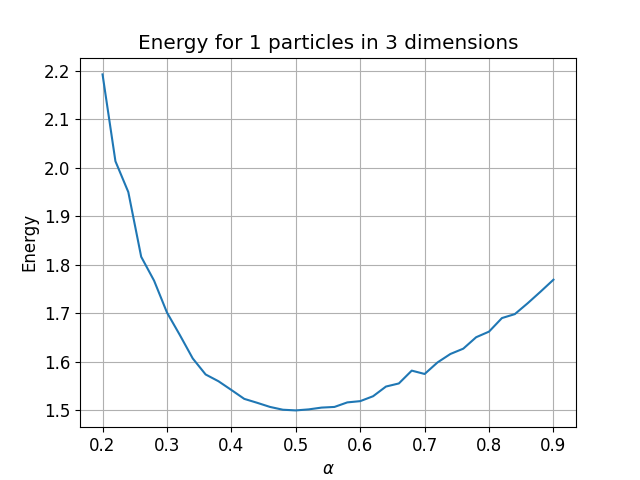
\includegraphics[width=\imwidth]{figures/Energy_C_1.png}
        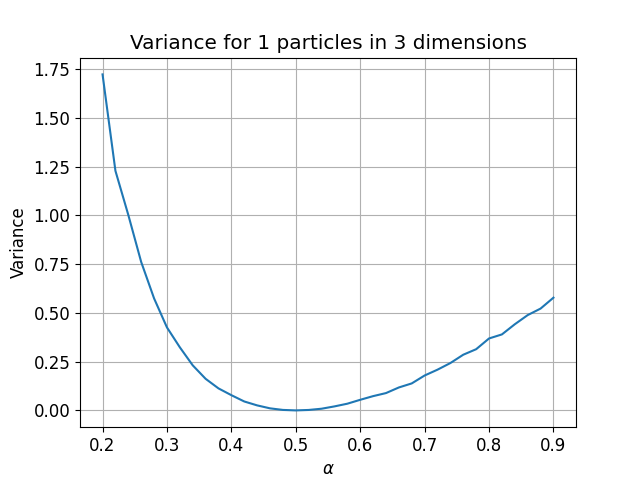
\includegraphics[width=\imwidth]{figures/Varience_C_1.png}
        \caption{Calcluated energy and variance using the Monte Carlo calculations with importance sampling for different values of the parameter $\alpha$ for $1$ non-interacing boson in a spherical trap.}
        \label{fig: C1}
    \end{figure}

    \begin{figure}[!ht]
        \centering
        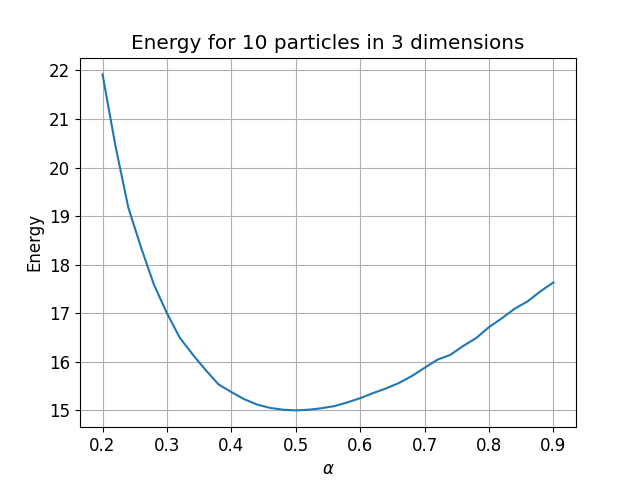
\includegraphics[width=\imwidth]{figures/Energy_C_10.png}
        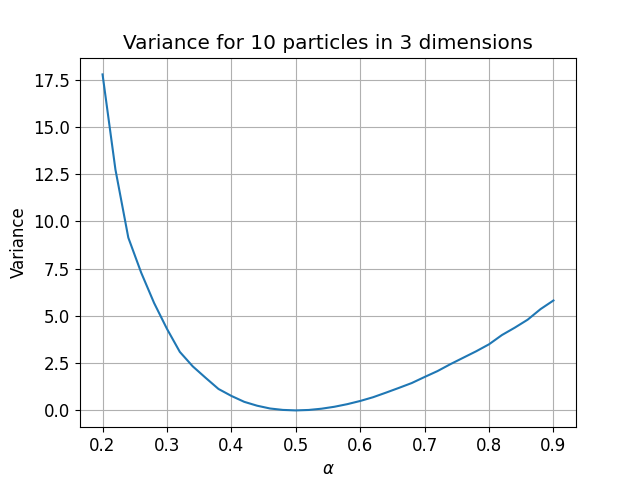
\includegraphics[width=\imwidth]{figures/Varience_C_10.png}
        \caption{Calcluated energy and variance using the Monte Carlo calculations with importance sampling for different values of the parameter $\alpha$ for $10$ non-interacing bosons in a spherical trap.}
        \label{fig: C10}
    \end{figure}

    \begin{figure}[!ht]
        \centering
        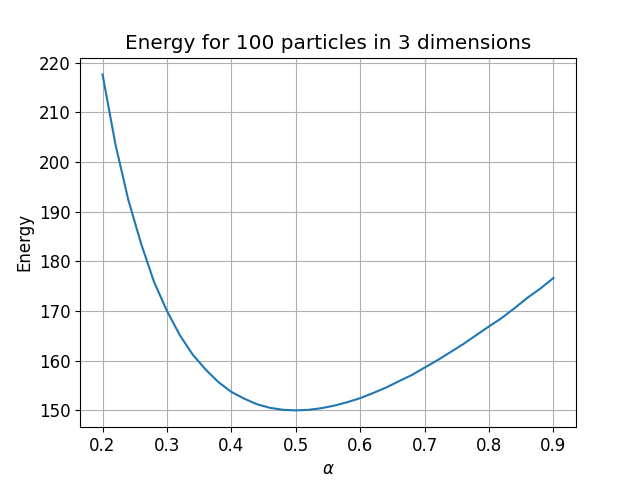
\includegraphics[width=\imwidth]{figures/Energy_C_100.png}
        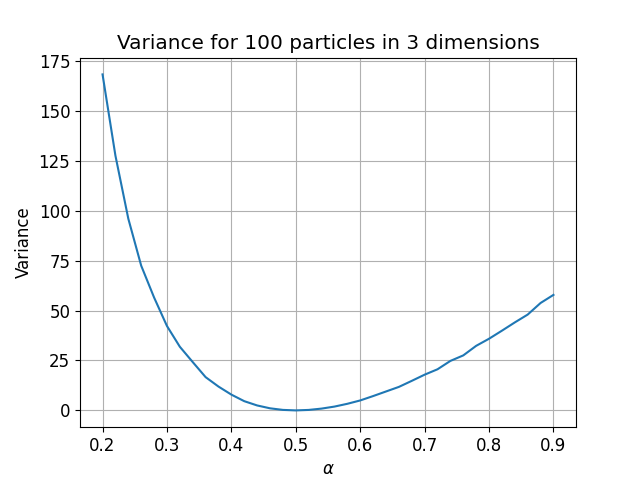
\includegraphics[width=\imwidth]{figures/Varience_C_100.png}
        \caption{Calcluated energy and variance using the Monte Carlo calculations with importance sampling for different values of the parameter $\alpha$ for $100$ non-interacing bosons in a spherical trap.}
        \label{fig: C100}
    \end{figure}
    
    \begin{figure}[!ht]
        \centering
        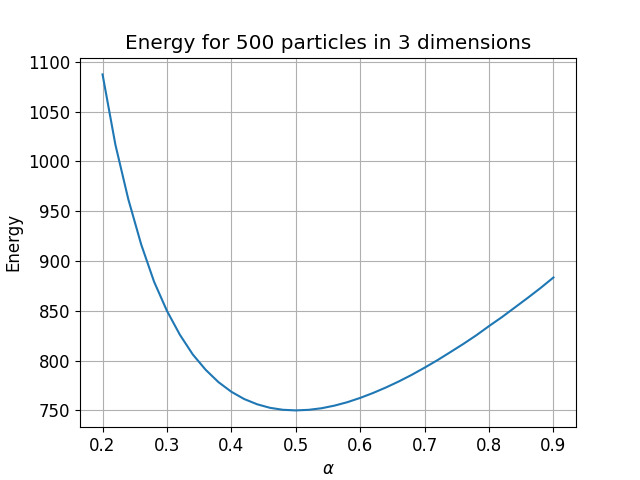
\includegraphics[width=\imwidth]{figures/Energy_C_500.png}
        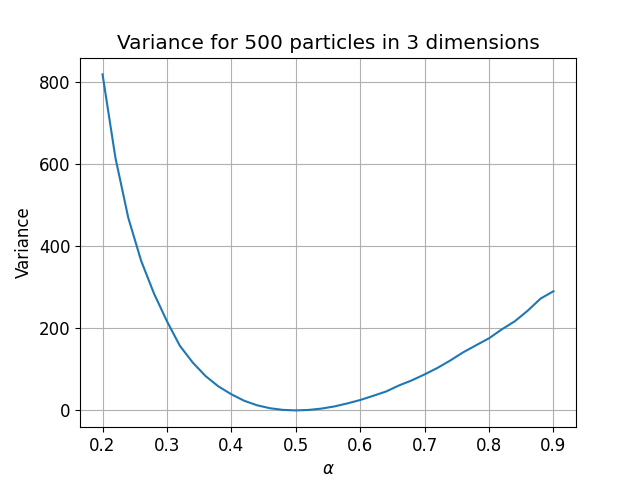
\includegraphics[width=\imwidth]{figures/Varience_C_500.png}
        \caption{Calcluated energy and variance using the Monte Carlo calculations with importance sampling for different values of the parameter $\alpha$ for $500$ non-interacing bosons in a spherical trap.}
        \label{fig: C500}
    \end{figure}\newpage
    
    \begin{table}[!ht]
        \begin{tabular}{|l|l|l|l|l|}
        \hline
                            & $n=1$         & $n=10$         & $n=100$         & $n=500$         \\ \hline
        Brute Force         & 29.43 seconds & 278.72 seconds & 2710.04 seconds & 13177.01 seconds\\ \hline
        Importance sampling & 4.36 seconds  & 42.01 seconds  & 409.61 seconds  & 2021.77 seconds \\ \hline
        \end{tabular}
        \caption{CPU time for a Monte Carlo calcualtion, with both equilibration steps and the main algorithm for $n=1$, $n=10$, $n=100$ and $n = 500$.}
        \label{table: time spent}
    \end{table}

    In the previous calculations we simply plotted the expectation values of the energies as a function of the parameter $\alpha$.
    For large systems this means that we spend equally many Monte Carlo cycles for values of $\alpha$ that are far away from the energy minimum as those that are close to it.
    To improve upon this we implement a steepest descent algorithm to minimize the energy and obtain the best possible value of $\alpha$.
    This algorithm is tested with a weight of $\eta = 0.01$, altough this was later changed to $\eta = 0.1/n$, for $n = 1$ in one dimension, $n = 2$ in two dimensions and $n = 3$ in three dimensions.
    The algorithm is stopped if the approximation for the energy derivative is lower than $10^{-4}$.
    For one particle in one dimension the algorithm reached $\alpha = 0.493966$ after 154 iterations.
    For two particles in two dimension the algorithm reached $\alpha = 0.4938934$ after 57 iterations.
    For three particles in three dimension the algorithm reached $\alpha = 0.499258$ after 23 iterations.

    In table \ref*{table: E} we see the results from the previously done calculations, with importance sampling, analysed using the blocking method.
    We note that the results largely match the analytic results and that the standard deviations are low inn all cases.
    The calcualtions are done for $n=1$, $n=10$, $n=50$ and $n=100$ with the values of alpha found with the gradient descent method.
    We can see that even with small variations in $\alpha$ the resulting energy is very close to the expected values at the optimal $\alpha = 0.5$.
    All computations that are shown in table \ref{table: E} have started with an initial guess for the variational paramet $\alpha = 0.4$.
    \begin{table}[!ht]
        \begin{tabular}{|l|l|l|l|}
        \hline
        Number of particles & Variational parameter $\alpha$    & Ground state energy   & Standard deviation    \\ \hline
        1                   & 0.498959                          & 1.500023              & 0.000037              \\ \hline
        10                  & 0.499256                          & 14.999892             & 0.000052              \\ \hline
        50                  & 0.495986                          & 75.001869             & 0.001104              \\ \hline
        100                 & 0.492543                          & 150.026922            & 0.002663              \\ \hline
        \end{tabular}
        \caption{Results from Monte Carlo calculation for non-interacting particles in a spherical trap.}
        \label{table: E}
    \end{table}

    Now that it is clear the calculations give the expected results for the non-interacting case we can move on to paralleize the code using OpenMP.
    The main idea behind the parallizition is to run the calculations several times averaging over the results.

    Then everything is ready for us to implement the repulsive interaction between particles.
    The trap used so far is converted to a elliptical one, described in eq \ref{eq: trap_eqn}.
    For conveniance we slightly restructure our Metropolis function to move a single particle at a time, rather than a single particle in a single dimension.
    This is done such that $f(a, \abs{r_i - r_j})$ can be calculated once rather than three times for each particle, in three dimensions. 


\section{\large The repuslive interaction}
    Table \ref{results 1} shows the results of our Monte Carlo calculation for an elliptical trap with $\beta = \gamma = 2.82843$ and $a/a_{ho} = 0.0043$ wiht $n=10$, $n=50$ and $n=100$ interacting particles.
    \begin{table}[!ht]
        \begin{tabular}{|l|l|l|l|}
        \hline
        Number of particles & Variational parameter $\alpha$    & Ground state energy   & standard deviation   \\ \hline
        10                  & 0.498085                          & 24.450653             & 0.027901             \\ \hline
        50                  & 0.493351                          & 129.103313            & 0.155081             \\ \hline
        100                 & 0.491609                          & 275.444469            & 0.01354              \\ \hline
        \end{tabular}
        \caption{Results from Monte Carlo calculation for interacting particles in a elliptical trap with $\beta = \gamma = 2.82843$ and $a/a_{ho} = 0.0043$.}
        \label{results 1}
    \end{table}
    Table \ref{results 2} shows the results of our Monte Carlo calculation for an elliptical trap with $\beta = \gamma = 2.82843$ with $n=10$, $n=50$ and $n=100$ non-interacting particles.
    \begin{table}[!ht]
        \begin{tabular}{|l|l|l|l|}
        \hline
        Number of particles & Variational parameter $\alpha$    & Ground state energy   & standard deviation   \\ \hline
        10                  & 0.5                               & 24.14405              & 0.000605             \\ \hline
        50                  & 0.5                               & 120.678625            & 0.027237             \\ \hline
        100                 & 0.5                               & 241.34062             & 0.065614             \\ \hline
        \end{tabular}
        \caption{Results from Monte Carlo calculation for non-interacting particles in a elliptical trap with $\beta = \gamma = 2.82843$ and $a/a_{ho} = 0.0043$.}
        \label{results 2}
    \end{table}
    The calculations are run using $2^{15}$ Monte Carlo cycles four times and then averaged.
    The optimization is run with $10^4$ Monte Carlo cycles for each value of $\alpha$.
    The number of equilibration steps is $10^4$.
    The number of Monte Carlo cycles is chosen as the sytems seem to equilibrate at a rapid pace such that running the calculations for longer wont change the results much.
    This can also be seen from the low standard deviations when calculating the energies.

    Comparing table \ref{results 1} and \ref{results 2} we note the increase in energy and decrease in the variational parameter $\alpha$ when we increase the number of particles.
    The increase in energy seems to match the results found in \cite{dubois2001bose}.
    The decrease in $\alpha$ matches the results from \cite{nilsen2005vortices}, altough in our case the change is rather small.

    \begin{table}[!ht]
        \begin{tabular}{|l|l|}
        \hline
                                                            & Onebody density                   \\ \hline
        Without repulsive interaction, $a=0$                & 0.702154 $\phi^2(\mathbf{r}_1)$   \\ \hline
        With repulsive interaction, $a/a_{ho} = 0.0043$     & 0.669945 $\phi^2(\mathbf{r}_1)$   \\ \hline
        \end{tabular}
        \caption{Calculated values for the onebody density for two particles, with and without the repulsive interaction.}
        \label{results 3}
    \end{table}
    In table \ref*{results 3} we see the results of the onebody calculations run for two particles with and without the repulsive interaction.
    We see that there is small decrease in the onebody density as a result of introducing the repulsive interaction.
    Yet it worth mentioning that runnung this calculation repeatedly gives slightly different results, however the overall result that the onebody density is higher without the repulse interaction stays prominent, although how much it changes from run to run varies.
    A statistical analysis of the onebody density should therefore be done, altough I do not have time for it at the current moment.
    
    
\section{Review of the project}
    Let us start with the positives.
    I feel like I have learned quite a few things working my way through this project.
    Programming in C++ is not something I have allot of experience in, and the class structures in this project was a good way of getting some hands on experience in how to write in this language.
    Furthermore it was a good introduction on how to think about coding projects, and how to plan ahead in your coding structure.
    I have learned allot through the mistakes that I made along the way and gotten a viewpoint of what aspects of the program should be prioritized when starting to write.

    Then to the negatives, of wich I only really have one.
    The pacing of this project seemed very off.
    It was in allot of ways very slow to start with until it all suddenly exploded towards the end.
    Some clearer goals of where you should be in the project at certain times would definately be appreaciated, and I believe it would be a good tool for knowing wich aspects that need to be shown in the lectures.

\bibliographystyle{plain}
\bibliography{Project_1}

\end{document}
